\section{ClangIR提出的背景}

\begin{frame}
    \frametitle{高层次信息的缺失}
    现代语言绝大部分编译器前端都设计了自己的 IR , FIR (Flang 的 IR ) 就是基于
    MLIR完成的。
    \begin{figure}[h]
        \centering
        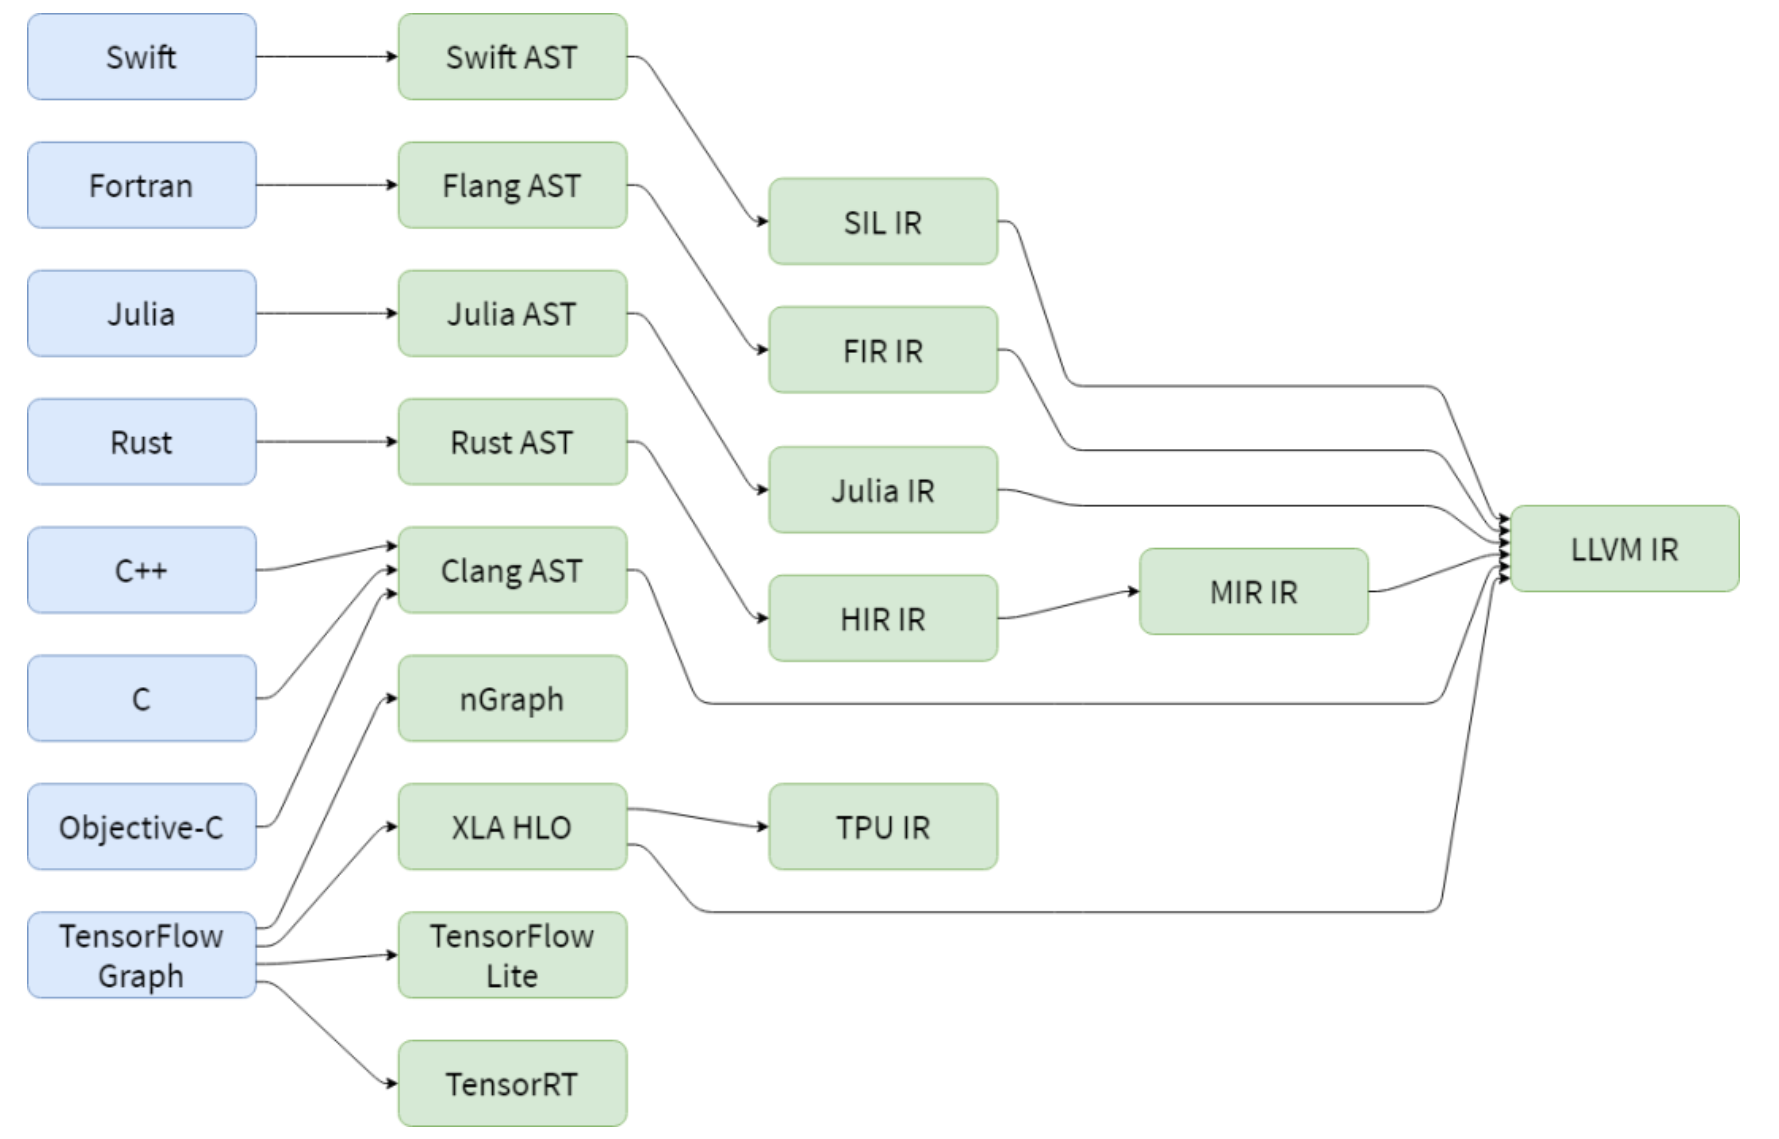
\includegraphics[width=0.45\textwidth]{images/compiler-ir.png}
        \caption{各大语言编译器前端使用 IR 的情况}
    \end{figure}

\end{frame}

\begin{frame}
    \frametitle{Clang 数据流分析诊断}

    Clang 的数据流相关诊断信息目前是在前端部分实现的。LLVM IR 更类似与一种三地
    址中间码,大量的信息会在 lower 到 LLVM IR 的路径中丢失。

    \begin{table}
        \centering
        \begin{tabular}{cc}
            \toprule
            已有的问题                             & 问题描述                                             \\
            \midrule
            \texttt{\_\_builtin\_constant\_p} & 与 LLVM 行为实际不一致\cite{aaronballman-constantp-2019} \\
            无穷递归                              & missing-warnings\cite{aaronballman-infrec-2019}  \\
            Lifetime                          & 难以实现                                             \\
            高层次的代码变换建议                        & 难以实现                                             \\
            \bottomrule
        \end{tabular}
        \caption{目前 Clang AST \& CFG 遇到的问题}
    \end{table}
    \label{tab:clang_diag}
\end{frame}

\begin{frame}[fragile]
    \frametitle{Infinite Recursive}
    \begin{center}
        \begin{minipage}{0.7\textwidth}
            \begin{lstlisting}[caption=无限递归诊断\cite{lyc-infrec-2019}]
void func1(int i) { /* no warning ?? */
    if (i || !i)
        func1(i);
}

void func2(int i) {
    if (i > 0 || i <= 0) /* tautological! */
       func2(i);
}
            \end{lstlisting}
        \end{minipage}
    \end{center}
\end{frame}

\begin{frame}[fragile]
    \frametitle{Lifetime}
    % TODO: 参考文献
    \begin{center}
        \begin{minipage}{0.8\textwidth}
            \begin{lstlisting}[caption=生命周期分析与垂悬引用]
int *p0() {
  int *p = nullptr;
  {
    int x = 0;
    p = &x;
    *p = 42;
  }        // note: pointee 'x' invalidated at end of scope
  *p = 42; // warning: use of invalid pointer 'p'
  return p;
}
            \end{lstlisting}

        \end{minipage}
    \end{center}

\end{frame}
